\lhead[\thepage]{CAPÍTULO \thechapter. ESTADO DEL ARTE}
\chead[]{}
\rhead[WepSIM: Simulador de procesador elemental con unidad de control microprogramada\leftmark]{\thepage}
\renewcommand{\headrulewidth}{0.5pt}

\lfoot[]{}
\cfoot[]{}
\rfoot[]{}
\renewcommand{\footrulewidth}{0pt}

%% This is an example first chapter.  You should put chapter/appendix that you
%% write into a separate file, and add a line \include{yourfilename} to
%% main.tex, where `yourfilename.tex' is the name of the chapter/appendix file.
%% You can process specific files by typing their names in at the 
%% \files=
%% prompt when you run the file main.tex through LaTeX.
\chapter{Estado del arte}
\label{ch:state_of_the_art}
\markboth{}{STATE OF THE ART}

Este capítulo presenta el estado del arte, la última y más avanzada etapa de las tecnologías relacionadas con nuestra aplicación. En primer lugar se presentan los diferentes simuladores existentes en el ámbito docente tanto para microprogramación (Section \ref{sec:simuladores_microprogramacion}) como para la programación en código ensamblador (Section \ref{sec:simuladores_ensamblador}), comparando una comparación de nuestro trabajo con el contexto actual de los distintos simuladores expuestos previamente (Section \ref{sec:propuesta_simulacion}). Después, se presentan las diferentes tecnologías web más utilizadas en la actualidad \ref{sec:tecnologias_web}. Por último se describe el procesador en el cual se basa WepSIM.

\section{Simuladores para la enseñanza de la Estructura y Arquitectura de Computadores}

Son muchos los tipos de simuladores existentes en el ámbito docente para la explicación de las distintas partes que componen un computador. Estos simuladores, pueden ser de diferentes ámbitos como por ejemplo, cachés, pipeline, circuitos integrados, microprogramación, programación en ensamblador, etc.

En este apartado, vamos a centrarnos en los tipos de simuladores que tienen relación directa con la propuesta realizada, como lo son los simuladores para la microprogramación y los simuladores para la programación en ensamblador.

\subsection{Simuladores para microprogramación}
\label{sec:simuladores_microprogramacion}

En esta sección, se explican los diferentes simuladores existentes para la microprogramación. Cabe destacar, que actualmente existen pocos simuladores que nos proporcionen esta funcionalidad, debido a que una gran parte de ellos, son utilizados de forma interna por las empresas para verificar el correcto funcionamiento de sus unidades en la fase de diseño y desarrollo. En primer lugar, vamos a centrarnos en los simuladores que están más enfocados a una labor docente.

P8080E \cite{p8080E} es un simulador desarrollado en el DATSI en la Facultad de Informática de la Universidad Politécnica de Madrid. Este simulador, no consta de una interfaz gráfica portable e interactiva que se ajuste a las tecnologías actuales. Para realizar poder realizar el desarrollo del microcódigo, el simulador requiere el binario completo de cada ciclo, de forma que resulta un tanto complejo su uso. Pese a ser un simulador bastante completo, no está orientado para la enseñanza de ensamblador y microprogramación con la misma herramienta, puesto que no permite la definición del juego de instrucciones con un formato diferente al definido por defecto.

\begin{figure}[htbp]
 	\centering
 	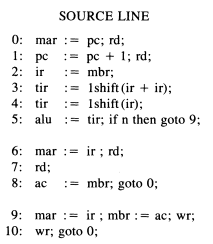
\includegraphics[width=6cm]{figures/ejemploTanenbaum}
 	\caption{Ejemplo de definición de microcódigo en simulador Tanenbaum.}
	\label{fig:tanenbaum_figure}
\end{figure}

En \cite{yen1986development}, se describe el desarrollo y la implementación de un simulador para una arquitectura de microprogramación específica. Fue publicado en el año 1986, y estaba basado en la arquitectura definida en el entonces popular libro de ingeniería de computadores \cite{tanenbaum1984}. El simulador, requería de la definición de cada uno de los ciclos de ejecución de las intrucciones para la posterior generación de la memoria de control. Esta definición, se realizaba mediante la sintaxis definida en el libro, lo que hacía de este simulador una herramienta bastante completa al para aprender junto con el libro. 


\subsection{Simuladores para programación en ensamblador}
\label{sec:simuladores_ensamblador}
En esta sección, se explican los diferentes simuladores existentes para la programación en ensamblador. Los simuladores más conocidos para labores docentes, son SPIM, MARS y WebMIPS.

\begin{figure}[htbp]
 	\centering
 	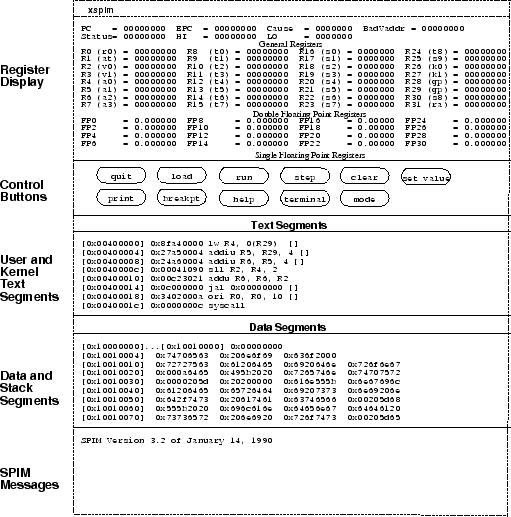
\includegraphics[width=8cm]{figures/spim_figure}
 	\caption{Interfaz SPIM.}
	\label{fig:spim_figure}
\end{figure}

SPIM \cite{larus1990spim}, es un simulador de un procesador MIPS de 32 bits desarrollado a principios de 1990. En un primer momento implementaba el juego de instrucciones MIPS-1, utilizado por los computadores MIPS R2000/R3000. Actualmente, implementa la arquitectura MIPS32 más reciente y sus instrucciones adicionales. Permite ejecutar programas en ensamblador para esta arquitectura. Además, también permite depurar el código implementado, de forma que el alumno pueda corregir con mayor facilidad los errores cometidos. Este simulador, fue creado por James R. Larus y tiene versiones compiladas para Windows, Mac OS X y Unix/Linux e incluso tiene una versión básica para Android, aunque su diseño no está pensado para dispositivos móviles. Puesto que el simulador está totalmente enfocado al procesador MIPS, posee el juego completo de instrucciones para la versión de 32 bits del procesador y todas las directivas de las que consta el lenguaje. Otra característica que hace de SPIM un potente simulador, es proveer de un pequeño sistema operativo que soporta las principales llamadas al sistema mediante la instrucción syscall. SPIM, es un simulador que permite múltiples configuraciones mediante su interfaz de usuario, de manera que se puede indicar:

\begin{itemize}

\item Activación del uso de pseudoinstrucciones.

\item Simulación de predicción de saltos y accesos a memoria, con la latencia correspondiente.

\item Activación del uso del manejador de la señal trap y la carga del manejador personalizado.

\item Activación de la visualización de los mensajes en caso de ocurrir excepciones.

\item Activación del uso de "memory-mapped IO".

\end{itemize}

SPIM, además cuenta con una versión más actualizada del simulador, que posee una interfaz gráfica más potente. Éste simulador se llama QtSPIM \cite{aguilar2013simuladores}, y cuenta con todas las características anteriormente mencionadas de SPIM.

\begin{figure}[htbp]
 	\centering
 	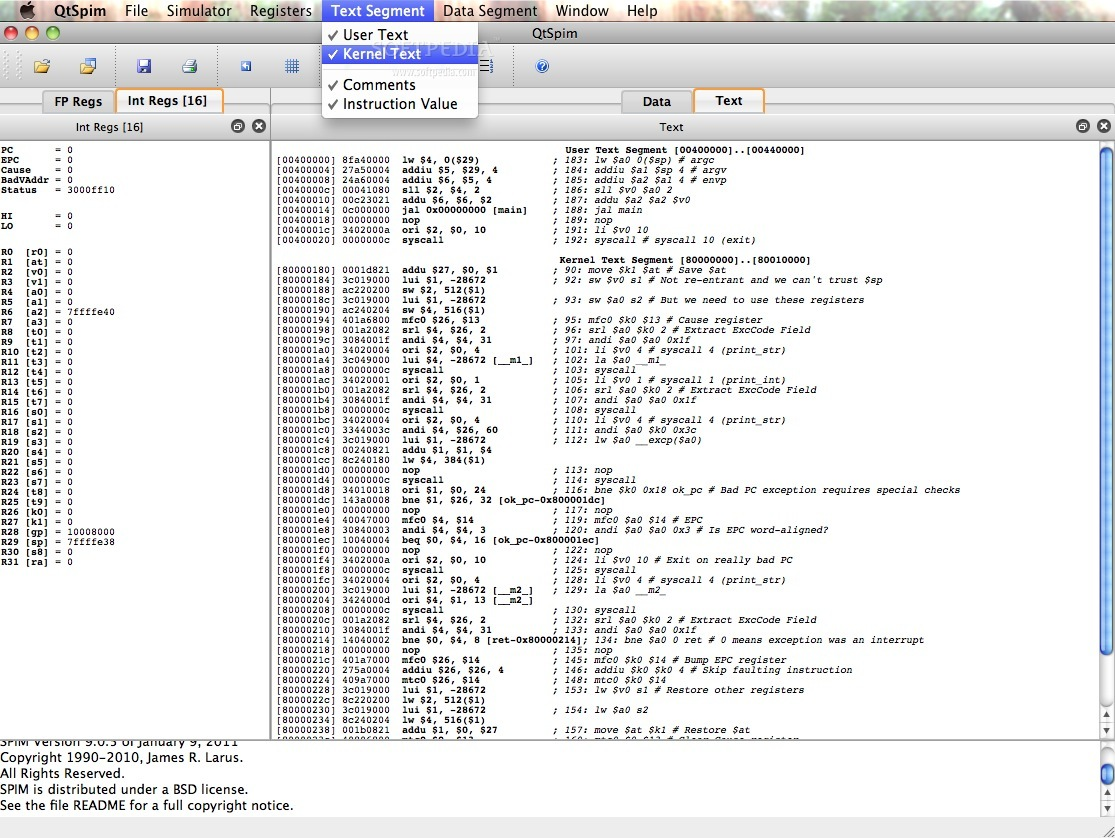
\includegraphics[width=12cm]{figures/qtspim_figure}
 	\caption{Interfaz QtSPIM.}
	\label{fig:qtspim_figure}
\end{figure}

MARS \cite{vollmar2006mars}, es un simulador con interfaz gráfica desarrollado en JAVA para el lenguaje ensamblador MIPS. Fue creado en el año 2005 como una alternativa del simulador SPIM y diseñado específicamente para las necesidades limitadas de cusos de pregrado. Está basado en la arquitectura MIPS RISC, que tiene un número pequeño de elementos del lenguaje e instrucciones. Consta de operaciones de entrada/salida, saltos, condiciones y operaciones aritmético-lógicas tanto enteras como en coma flotante. Alguna de las mejoras que incorpora MARS con respecto a SPIM son \cite{vegdahl2008mipspilot}: 

\begin{itemize}

\item Depuración más sencilla y cómoda, debido constar de GUI. Ésto se debe, a que para añadir un punto de ruptura, únicamente hay que clickar sobre un checkbox que tiene la instrucción.

\item Los programas puedes ejecutarse de forma inversa, lo que permite volver a un estado anterior de la máquina en la ejecución de un programa.

\item La velocidad de ejecución puede modificarse, de forma que si se ralentiza el usuario puede observar como cada instrucción se resalta cuando está siendo ejecutada y ver los cambios que se producen en los valores del banco de registros y de las ubicaciones de memoria.

\item  La memoria y los registros se pueden modificar de una manera WYSIWYG.

\item Incorpora un editor de texto, eliminando dependencias externas para el uso del simulador.

\item Permite que los desarrolladores puedan suministrar nuevos complementos, que por ejemplo, sirvan para extender la arquitectura o mostrar los datos de forma intuitiva.

\end{itemize}

\begin{figure}[htbp]
 	\centering
 	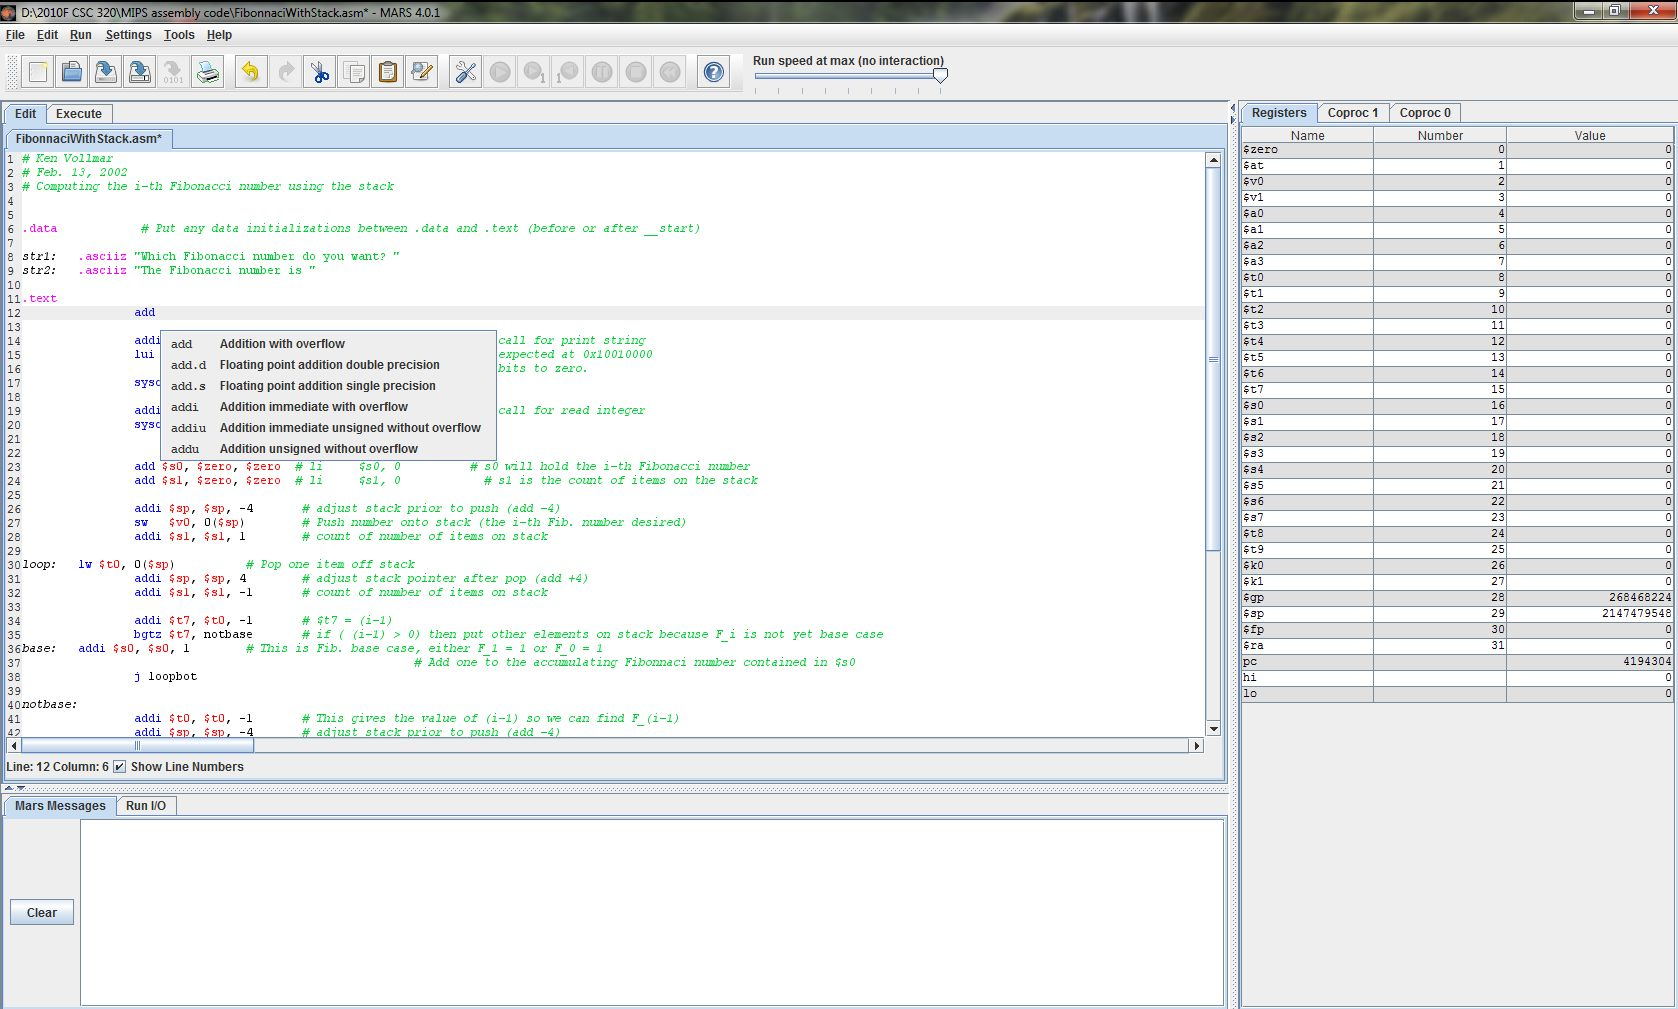
\includegraphics[width=14cm]{figures/mars_figure}
 	\caption{Interfaz MARS.}
	\label{fig:mars_figure}
\end{figure}

P88110, es emulador descrito en \cite{garcia2009p88110} que se basa en la emulación de un procesador superescalar. El propósito fundamental de este emulador, es mostrar el funcionamiento de este tipo de procesadores, haciendo visible el funcionamiento del pipeline y las dependencias existentes. Está basado en una arquitectura específica (MC88110) y pese a integrar el efecto de un procesador superescalar no integra la microprogramación, que haría de él un emulador completo.

\begin{figure}[htbp]
 	\centering
 	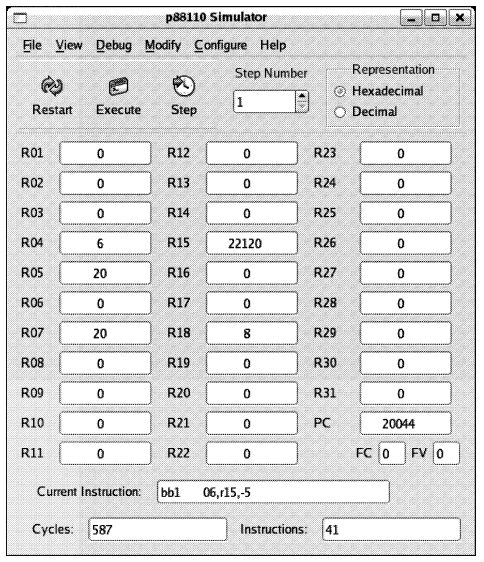
\includegraphics[width=8cm]{figures/em88110}
 	\caption{Interfaz em88110.}
	\label{fig:p88110_figure}
\end{figure}


WebMIPS \cite{branovic2004webmips}, es un simulador desarrollado en la Facultad de Ingeniería de la Información de Sienna, Italia. Está escrito en el lenguaje de programación ASP.NET y se utiliza mediante una página web, de forma que no requiere de su instalación en local. No soporta el juego completo de instrucciones de MIPS, sino que consta de un juego reducido de instrucciones que sirve de intruducción al estudio de arquitectura de computador. Con respecto a los anteriores simuladores mencionados, difiere al mostrar el esquema arquitectónico, indicando las 5 etapas de pipeline de las que consta el computador que simula. Otra característica, es la indicación del número de ciclos de reloj que consume la ejecución del programa. Tiene como objetivo principal la demostración de la ejecución del juego de instrucciones básico explicado durante la asignatura "Arquitectura de Computadores" impartida por los creadores del simulador.

Entre las diferentes características a destacar de este simulador, se encuentran:

\begin{itemize}
	
\item Verificación del código ensamblador, comprobando que no existen errores en la definición el código.

\item Dispone de códigos simples de ejemplo ("load-and-play") que facilitan la comprensión del funcionamiento del procesador.

\item Permite diferentes visualizaciones del estado de la memoria y los registros del procesador.

\item Consta de dos modos de ejecución: paso a paso y ejecución completa del programa.
	
\end{itemize}

\begin{figure}[htbp]
 	\centering
 	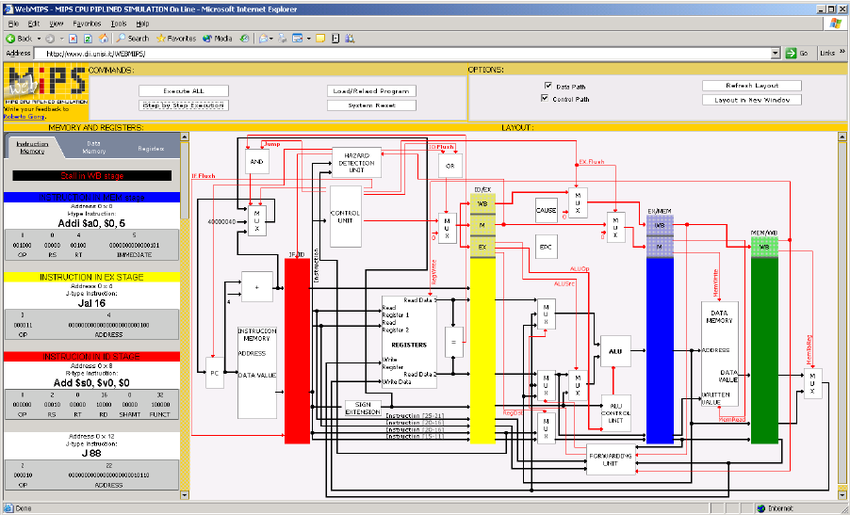
\includegraphics[width=15cm]{figures/webmips_figure}
 	\caption{ Interfaz WebMIPS.}
	\label{fig:webmips_figure}
\end{figure}

\clearpage

\subsection{Propuesta de simulación unificada}
\label{sec:propuesta_simulacion}
Hay distintas herramientas muy útiles para labores docentes relacionadas con la asignatura Estructura de Computadores, aunque como se comento previamente, no existe una herramienta que nos proporcione el desarrollo y simulación tanto a nivel de microcódigo como a nivel de ensamblador. WepSIM, une ambos aspectos ofreciendo:

\begin{itemize}
	\item Visión interrelacionada de la microprogramación y la programación en ensamblador.
	\item Flexibilidad en la plataforma usada, pensando el dispositivos móviles.
	\item Herramienta autocontenida, de forma que incorpora en sí misma tanto la ayuda como distintos ejemplos que favorecen la comprensión del simulador.
	\item Consta de un modelo hardware que puede ser modificado o ampliado en caso de ser necesario.
	\item Permite definir un amplio conjunto de instrucciones máquina.
	\item Puede ser usado como herramienta de microprogramación o de programación en ensamblador.
\end{itemize}

\begin{table}[htbp]
\ra{1.2}
\centering
%\resizebox{\textwidth}{%
\resizebox{\textwidth}{!}{
\begin{tabular}{@{}llllllll@{}}
\toprule
Simulador & SPIM & MARS & PC88110 & WebMIPS & WepSIM  & P8080E & MicMac\\ 
\midrule
Ensamblador				& \ding{51} & \ding{51} & \ding{51} & \ding{51} & \ding{51} &  &  \\
\midrule
Microprogramación				&  &  &  &  & \ding{51} & \ding{51} & \ding{51} \\
\midrule
Multiplataforma				& \ding{51} &  &  & \ding{51} & \ding{51} &  &  \\
\midrule
Interactivo				&  &  &  &  & \ding{51} &  &  \\
\midrule
Juego de instrucciones personalizable				&  &  &  &  & \ding{51} &  &  \\
\bottomrule
\end{tabular}
}
\caption{Comparación de simuladores de ensamblador y microcódigo.}
\label{tab:comparison_frameworks}
\end{table}

De este modo, con WepSIM se pretende crear un simulador unificado, abarcando los aspectos más relevantes de la asignatura 'Estructura de Computadores' y permitiendo que todas las prácticas de la asignatura puedan realizarse en la misma plataforma, evitando la pérdida de tiempo y dificultad que supone para el alumno el habituarse a diferentes entornos para cada una de las prácticas.

WepSIM, se puede definir por tanto como un simulador de programación en ensamblador y microprogramación, flexible puesto que permite la personalización del juego de instrucciones de la máquina, multiplataforma puesto que permite su uso desde diferentes tipos de dispositivos, e interactivo al poder modificar la configuración de la máquina en tiempo de ejecución.


\section{Tecnologías web}
\label{sec:tecnologias_web}

Actualmente, gran parte de los recursos disponibles en el día a día son ofrecidos a través de Internet y su distribución es posible gracias a las tecnologías web. Estas tecnologías, permiten la construcción de las páginas web haciendo uso de las tecnologías para el desarrollo de páginas web y las tecnologías de interconexión de computadores permitiendo a los usuarios el intercambio en formato de hipertexto de todo tipo de datos y de aplicaciones software.

\subsection{HTML5}
\label{sec:html5}

Cuando se realiza el desarrollo de una página web, son tres las tecnologías que se emplean con mayor frecuencia: HTML, CSS y JavaScript. Todas estas tecnologías vienen definidas y estandarizadas por el organismo internacional W3C y cada una de ellas, tiene una función concreta en el funcionamiento de la página web:

\begin{itemize}
\item \textbf{HTML}: Es un lenguaje de marcado con el que se realiza la estructuración de la página web. Es un estándar que sirve de referencia del software que conecta con la elaboración de páginas web en sus diferentes versiones, define una estructura básica y un código (denominado código HTML) para la definición de contenido de una página web, como texto, imágenes, vídeos, juegos, entre otros. 

El lenguaje HTML basa su filosofía de desarrollo en la diferenciación. Para añadir un elemento externo a la página (imagen, vídeo, script, entre otros.), este no se incrusta directamente en el código de la página, sino que se hace una referencia a la ubicación de dicho elemento mediante texto. De este modo, la página web contiene solamente texto mientras que recae en el navegador web (interpretador del código) la tarea de unir todos los elementos y visualizar la página final. Al ser un estándar, HTML busca ser un lenguaje que permita que cualquier página web escrita en una determinada versión, pueda ser interpretada de la misma forma (estándar) por cualquier navegador web actualizado.

En cambio, a lo largo de las diferentes versiones, se han añadido y eliminado diferentes características, con la finalidad de hacer el lenguaje más eficiente y facilitar el desarrollo de páginas web con diferentes plataformas y navegadores. Un navegador web  desactualizado, no será capaz de interpretar correctamente una página web escrita en una versión superior de HTML a la que pueda interpretar.  

\item \textbf{CSS}: Es un lenguaje de diseño gráfico utilizado para definir y crear la presentación de un documento estructurado escrito en un lenguaje de marcado, como puede ser, HTML. Su principal finalidad, es establecer el diseño visual de las páginas web e interfaces de usuario escritas en los lenguajes HTML o XHTML. Este lenguaje además, permite aplicar estilos no visuales como pueden ser las hojas de estilo auditivas.

Esta tecnología web, es usada por la mayoría de sitios web para crear páginas visualmente atractivas, interfaces de usuario para aplicaciones web, y GUIs para muchas de las aplicaciones móviles existentes en el mercado. Con ella, se pretende separar el contenido de la página web de la presentación, buscando mejorar la accesibilidad del documento y dando una mayor flexibilidad y control en la especificación de las características de la presentación, permitiendo que varios docuementos HTML compartan un mismo estilo usando una única hoja de estilos reduciendo la complejidad y la repetición de código en la estructura del documento.

\item \textbf{JavaScript}: Es un lenguaje de programación interpretado orientado a las páginas web que surgió de la necesidad de ampliar las posibilidades del HTML. Su principal función en las páginas web, es realizar tareas y operaciones en el marco de la aplicación cliente como la mejora de la interfaz de usuario y la generación de páginas web dinámicas, aunque también es utilizado en el lado del servidor .

Este lenguaje, fue diseñado con una sintaxis similar a la del lenguaje de programación C, aunque adopta nombres y convenciones del lenguaje de programación Java. En cambio, Java y Javascript tienen propósitos y semánticas distintos.

En la actualidad, todos los navegadores realizan la interpretación del código JavaScript integrado en las páginas web. Para poder interactuar con una página web el lenguaje está provisto de una implementación del DOM que facilita el control y manejo de las interacciones del usuario.

\end{itemize}

\subsection{Frameworks}
\label{sec:frameworks}

Como se indica en \cite{garrido2004arquitectura} las aplicaciones web se han convertido en los últimos años en complejos sistemas software con interfaces de usuario cada vez más parecidas a las aplicaciones de escritorio, dando servicio a procesos de negocio de considerable envergadura y estableciéndose sobre ellas requisitos estrictos de accesibilidad y respuesta. Para ayudar al desarrollo de estas aplicaciones web, se hace uso de diferentes frameworks y bibliotecas que añaden funcionalidad al entorno de trabajo. Los frameworks son una estructura conceptual para el desarrollo e implementación de aplicaciones web, teniendo como objetivos principales la aceleración del proceso de desarrollo, reutilización de código ya existente y promover buenas prácticas de desarrollo, como el uso de patrones. Entre los frameworks más utilizados en la actualidad, se encuentran:

\begin{itemize}

\item \textbf{Angular.js}: Es un framework MVC (Modelo-Vista-Controlador) de JavaScript de código abierto mantenido por Google para el desarrollo Web Front End, que permite crear aplicaciones \textit{Single-Page}. Este framework ha supuesto un avance puesto que al implementar el patrón MVC ayuda al desarrollador a separar conceptos. De este modo, adapta y amplía el HTML tradicional para servir mejor contenido dinámico a través de un \textit{data binding} bidireccional que permite la sincronización automática de modelos y vistas. Además facilita la creación de test unitarios, lo cual resulta de gran ayuda para los desarrolladores.

\item \textbf{jQuery.js}: Es una biblioteca de JavaScript rápida, pequeña y característica. Ofrece una infraestructura que proporciona una mayor facilidad para la creación de aplicaciones complejas del lado del cliente. De esta forma, al utilizar esta biblioteca, el desarrollador se asegura que funcionará correctamente en los navegadores de los usuarios.

\item \textbf{BootStrap}: Es un framework de código abierto para el diseño de aplicaciones web, en el cual se incluyen diferentes plantillas de diseño con tipografía, formularios, botones, menús de navegación y otros elementos de diseño basados en HTML y CSS que proporcionan el desarrollador ayuda a la hora de implementar la interfaz de usuario de su aplicación. Además, es compatible con la mayoría de los navegadores web.

\item \textbf{Dojo}: Es un framework que contiene APIs que facilitan el desarrollo de aplicaciones web que utilizan la tecnología AJAX, conteniendo un sistema de empaquetado inteligente, efecto de interfaz de usuario, abstracción de eventos, almacenamiento de APIs en el cliente e interacción de APIs con AJAX.

\end{itemize}

\section{Procesador elemental WepSIM}

WepSIM, es un procesador elemental con unidad de control microprogramada diseñado por el personal del grupo de investigación ARCOS de la Universidad Carlos III de Madrid para la docencia en la asignatura Estructura de Computadores.

En la figura \ref{fig:wepsimCPU_figure}, se muestra la estructura del Procesador Elemental WepSIM. WepSIM, consta de un módulo de memoria, un dispositivo teclado, un dispositivo pantalla y un dispositivo de E/S genérico que se puede utilizar para trabajar con interrupciones.

\begin{figure}[htbp]
 	\centering
 	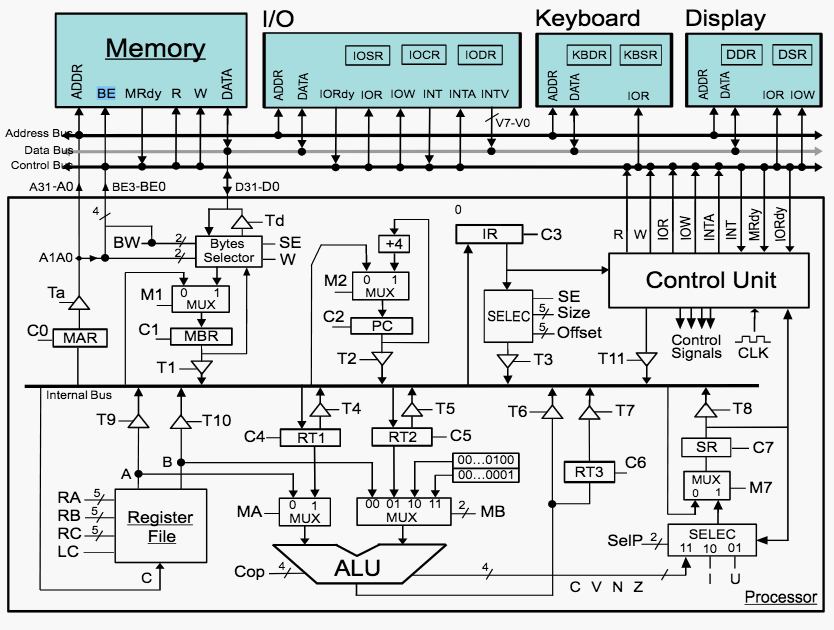
\includegraphics[width=11cm]{figures/cpu}
 	\caption{Arquitectura CPU WepSIM .}
	\label{fig:wepsimCPU_figure}
\end{figure}

\begin{figure}[htbp]
 	\centering
 	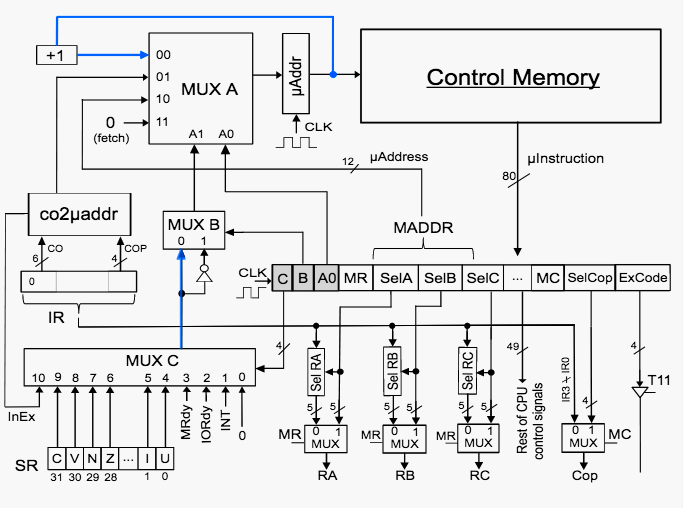
\includegraphics[width=11cm]{figures/controlUnit}
 	\caption{Arquitectura unidad de control WepSIM.}
	\label{fig:wepsimCU_figure}
\end{figure}

WepSIM es un procesador de 32 bits que direcciona la memoria por bytes, que cuenta con un banco de 32 registros y dos registros adicionales (RT1 y RT2) que no son visibles para el programador de ensamblador, pero que permiten el almacenamiento temporal de datos para la realización de operaciones intermedias. Desde los registros, es posible enviar los valores para operar en una ALU que dispone de las 15 operaciones aritmético-lógicas más comunes. El registro PC tiene su propio operador de sumar cuatro, de forma que no es necesario hacer uso de la ALU para esta operación. El resultado de las operaciones realizadas en la ALU puede ser almacenado en un registro temporal (RT3) que también es invisible para el programador de ensamblador, o ser enviado directamente al bus interno a través del correspondiente triestado.

El registro de estado (SR) puede ser actualizado con los flags resultantes de la última operación de la alu (O, N y Z). Para ello, SELEC/SelP representa un bloque de circuitos que permite indicar qué parte del registro de estado (SR) debe ser actualizado. A la derecha de SELEC/SelP llegan los bits del registro de estado SR como entrada (Input=O N Z I U) y SelP permite seleccionar qué grupo de estos bits se actualizará en el registro de estado: los bits O, N y Z con los valores procedentes de la ALU, el bit I con el valor indicado o el bit U con el valor indicado para el mismo.

El registro de instrucción (IR) tiene asociado un módulo selector (circuito de  más alto nivel que un multiplexor, etc.) que permite seleccionar un segmento del valor binario almacenado en el registro de instrucción que pasará hacia T3.

En concreto, se indica la posición (Offset, donde 0 represente el bit menos significativo del registro IR) inicial y el número de bits (Size) a tomar a partir de dicha posición inicial, así como si se desea hacer extensión de signo (SE) antes de pasar el valor a la entrada de T3.

Los registros MAR y MBR se usan para almacenar la dirección y el contenido asociado a esta dirección en las operaciones de lectura/escritura con la memoria. La memoria está diseñada para un funcionamiento síncrono o asíncrono. Actualmente funciona de forma síncrona, pero dispone de la señal MRdy para en un futuro trabajar de forma asíncrona. El circuito de selección permite indicar qué porción de la palabra de memoria es la que se desea (un byte, dos bytes o una palabra completa de cuatro bytes).

Se dispone también de tres dispositivos de E/S: un teclado, una pantalla y un dispositivo genérico que se puede configurar para generar diversos tipos de interrupciones.

Finalmente, la Unidad de Control genera las señales de control para cada ciclo de reloj. La figura \ref{fig:wepsimCU_figure} muestra la Unidad de Control con mayor detalle. Se trata de una unidad de control microprogramada con secuenciamiento implícito. Las señales de control para el ciclo de reloj actual se almacenan en el registro de micro-instrucción (aquel con los campos A0, B, C, SelA, etc.). El contenido de este registro proviene de la memoria de control, concretamente del contenido en la posición a la que apunta el registro de micro-dirección. La micro-dirección almacenada en este registro puede modificarse usando el multiplexor "MUX A". Hay cuatro opciones: la microdirección actual más uno, una micro-dirección indicada en la propia micro-instrucción (que se solapa con SelA, SelB y parcialmente con SelE), la primera micro-dirección asociada al campo de código de operación de la instrucción del registro IR, y finalmente el valor cero, que es la dirección de la memoria de control donde se almacena la microrrutina correspondiente al fetch. La microdirección se puede seleccionar de forma condicional, para ello se usa el multiplexor "MUX C" que permite seleccionar los bits del registro de estado (SR) o valores de las señales de control de E/S.

Para generar los valores correspondientes a las señales selectoras del banco de registros RA, RB y RE se usan los circuitos selectores SelRA, SelRB y SelRE. Estos selectores toman como entrada los 32 bits del registro de instrucción (IR) por un lado y el campo SelA, SelB y SelE por otro, de forma que toman SelX como el desplazamiento dentro del registro de instrucción (de 0 a 32) desde donde tomar los siguientes 5 bits correspondientes a las señales RA, RB o RE. Permiten por tanto seleccionar 5 bits consecutivos de los 32 bits del registro de instrucción.

El multiplexor MR permite indicar si las señales RA, RB y RE serán literalmente los valores almacenados en SelA, SelB y SelE (MR=1) o bien si SelA, SelB y SelE indican el desplazamiento dentro de la instrucción donde están los valores a utilizar para RA, RB y RE. Esto último permite que en la instrucción se pueda indicar los registros a usar como operandos en el banco de registros, en lugar de indicarlos desde la micro-instrucción.

Para la señal Cop (código de operación en la ALU) la señal MC permite tomar el valor SelCop de la micro-instrucción (MC=1) o bien los 4 bits menos significativos del registro de instrucción (MC=0), es decir IR3-IR0.

En \cite{perez2015problemas} se puede encontrar una descripción más detallada del procesador descrito anteriormente.





